\documentclass{article}
\usepackage{verbatim}
\usepackage{graphics}
\usepackage{tikz}
\usepackage{pgfplots}

\pgfrealjobname{minimal}

\begin{document}

\beginpgfgraphicnamed{figure}
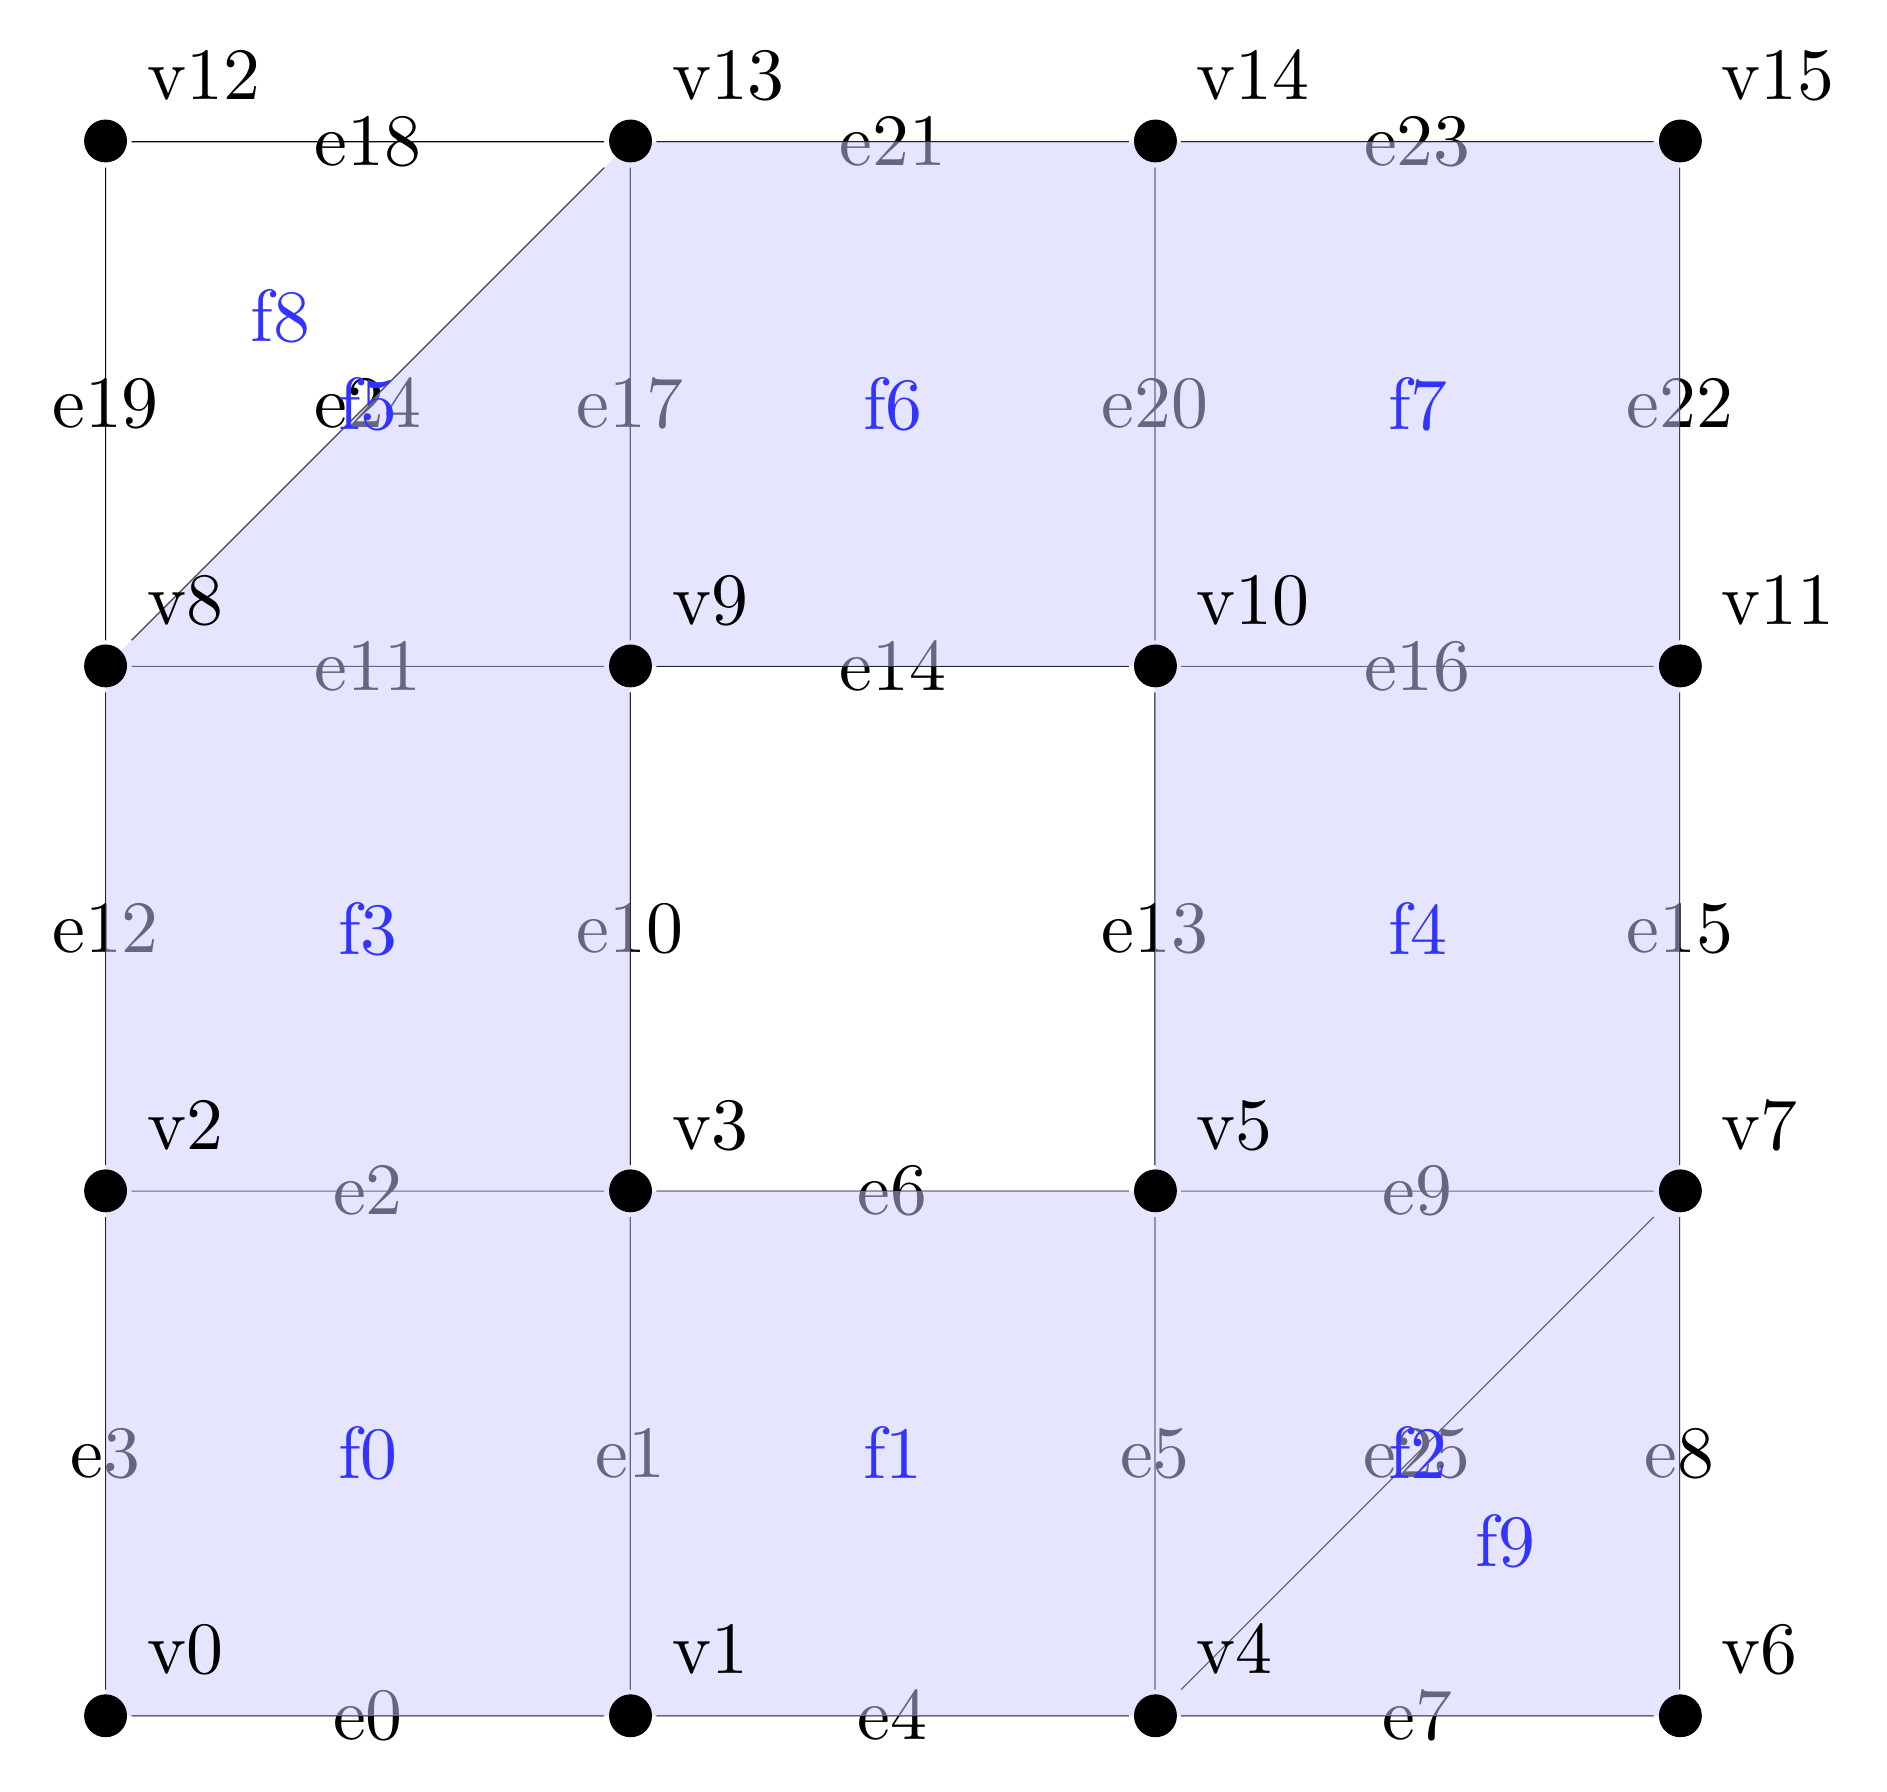
\begin{tikzpicture}[scale=6.666667, every node/.style={scale=2.666667}]

%vertex labels
\draw
	(0.000000,0.000000) node (v0) {}
	(1.000000,0.000000) node (v1) {}
	(0.000000,1.000000) node (v2) {}
	(1.000000,1.000000) node (v3) {}
	(2.000000,0.000000) node (v4) {}
	(2.000000,1.000000) node (v5) {}
	(3.000000,0.000000) node (v6) {}
	(3.000000,1.000000) node (v7) {}
	(0.000000,2.000000) node (v8) {}
	(1.000000,2.000000) node (v9) {}
	(2.000000,2.000000) node (v10) {}
	(3.000000,2.000000) node (v11) {}
	(0.000000,3.000000) node (v12) {}
	(1.000000,3.000000) node (v13) {}
	(2.000000,3.000000) node (v14) {}
	(3.000000,3.000000) node (v15) {};

%plot non-open edges
\draw
	(v0)--(v1) node [midway] {e0}
	(v1)--(v3) node [midway] {e1}
	(v3)--(v2) node [midway] {e2}
	(v2)--(v0) node [midway] {e3}
	(v1)--(v4) node [midway] {e4}
	(v4)--(v5) node [midway] {e5}
	(v5)--(v3) node [midway] {e6}
	(v4)--(v6) node [midway] {e7}
	(v6)--(v7) node [midway] {e8}
	(v7)--(v5) node [midway] {e9}
	(v3)--(v9) node [midway] {e10}
	(v9)--(v8) node [midway] {e11}
	(v8)--(v2) node [midway] {e12}
	(v5)--(v10) node [midway] {e13}
	(v10)--(v9) node [midway] {e14}
	(v7)--(v11) node [midway] {e15}
	(v11)--(v10) node [midway] {e16}
	(v9)--(v13) node [midway] {e17}
	(v13)--(v12) node [midway] {e18}
	(v12)--(v8) node [midway] {e19}
	(v10)--(v14) node [midway] {e20}
	(v14)--(v13) node [midway] {e21}
	(v11)--(v15) node [midway] {e22}
	(v15)--(v14) node [midway] {e23}
	(v13)--(v8) node [midway] {e24}
	(v7)--(v4) node [midway] {e25};

%plot open edges
\draw[very thick, dashed];

%fill faces
\fill[color=blue!20, opacity=.5] 
	(v0.center)--(v1.center)--(v3.center)--(v2.center)--cycle
	(v1.center)--(v4.center)--(v5.center)--(v3.center)--cycle
	(v4.center)--(v6.center)--(v7.center)--(v5.center)--cycle
	(v3.center)--(v2.center)--(v8.center)--(v9.center)--cycle
	(v7.center)--(v5.center)--(v10.center)--(v11.center)--cycle
	(v9.center)--(v8.center)--(v12.center)--(v13.center)--cycle
	(v10.center)--(v9.center)--(v13.center)--(v14.center)--cycle
	(v11.center)--(v10.center)--(v14.center)--(v15.center)--cycle
	(v12.center)--(v8.center)--(v13.center)--cycle
	(v4.center)--(v6.center)--(v7.center)--cycle;

%plot faces indices
\draw
   (0.500000,0.500000) node[color=blue!80] {f0}
   (1.500000,0.500000) node[color=blue!80] {f1}
   (2.500000,0.500000) node[color=blue!80] {f2}
   (0.500000,1.500000) node[color=blue!80] {f3}
   (2.500000,1.500000) node[color=blue!80] {f4}
   (0.500000,2.500000) node[color=blue!80] {f5}
   (1.500000,2.500000) node[color=blue!80] {f6}
   (2.500000,2.500000) node[color=blue!80] {f7}
   (0.333333,2.666667) node[color=blue!80] {f8}
   (2.666667,0.333333) node[color=blue!80] {f9};

%vertex indices
\draw
	(0.000000,0.000000) node[draw, circle, inner sep=2pt, fill=black, label = above right:v0] () {}
	(1.000000,0.000000) node[draw, circle, inner sep=2pt, fill=black, label = above right:v1] () {}
	(0.000000,1.000000) node[draw, circle, inner sep=2pt, fill=black, label = above right:v2] () {}
	(1.000000,1.000000) node[draw, circle, inner sep=2pt, fill=black, label = above right:v3] () {}
	(2.000000,0.000000) node[draw, circle, inner sep=2pt, fill=black, label = above right:v4] () {}
	(2.000000,1.000000) node[draw, circle, inner sep=2pt, fill=black, label = above right:v5] () {}
	(3.000000,0.000000) node[draw, circle, inner sep=2pt, fill=black, label = above right:v6] () {}
	(3.000000,1.000000) node[draw, circle, inner sep=2pt, fill=black, label = above right:v7] () {}
	(0.000000,2.000000) node[draw, circle, inner sep=2pt, fill=black, label = above right:v8] () {}
	(1.000000,2.000000) node[draw, circle, inner sep=2pt, fill=black, label = above right:v9] () {}
	(2.000000,2.000000) node[draw, circle, inner sep=2pt, fill=black, label = above right:v10] () {}
	(3.000000,2.000000) node[draw, circle, inner sep=2pt, fill=black, label = above right:v11] () {}
	(0.000000,3.000000) node[draw, circle, inner sep=2pt, fill=black, label = above right:v12] () {}
	(1.000000,3.000000) node[draw, circle, inner sep=2pt, fill=black, label = above right:v13] () {}
	(2.000000,3.000000) node[draw, circle, inner sep=2pt, fill=black, label = above right:v14] () {}
	(3.000000,3.000000) node[draw, circle, inner sep=2pt, fill=black, label = above right:v15] () {};

\end{tikzpicture}
\endpgfgraphicnamed

\end{document}
